\documentclass[12pt, a4paper]{article}
\usepackage[margin=1in]{geometry}
\usepackage{graphicx}
\usepackage{float}
\usepackage{booktabs}
\usepackage{hyperref}
\setlength{\parindent}{0pt}
\setlength{\parskip}{0.5pt}

\title{
    \vspace{-1cm}
    \Large\textbf{Bike Sharing Demand Forecasting:\\OLS, Ridge, and Lasso Analysis}
}
\author{
    William Chen
}
\date{}

\begin{document}
\maketitle
\thispagestyle{empty}

%-----------------------------------------------------------------------
\begin{abstract}
This report analyses daily bike rental demand using the UCI Bike Sharing
Dataset, comprising 731 observations collected from the Capital Bikeshare
system in Washington, D.C. between 2011 and 2012. We apply Ordinary Least Squares (OLS) regression as the primary model,
and compare it against Ridge and Lasso regression to evaluate the effect
of regularisation. Following careful feature selection and
multicollinearity diagnostics, the final model is trained on 8 predictors
spanning temporal, weather, and calendar dimensions.
 
The OLS model achieves an in-sample $R^2$ of 0.827 and a 5-fold
cross-validated RMSE of 821, outperforming Ridge (835) and Lasso (831).
Year and temperature emerge as the strongest predictors. Residual
diagnostics confirm that linear model assumptions are largely satisfied,
with only mild heteroscedasticity observed at higher fitted values.
\end{abstract}
\newpage
%-----------------------------------------------------------------------
\section{Introduction}

Bike-sharing systems have become an increasingly popular form of urban
transportation, offering a flexible and environmentally friendly alternative
to private vehicles. Accurately forecasting daily rental demand is valuable
for operators seeking to optimise fleet distribution, staffing, and
infrastructure planning. Demand is inherently influenced by a combination
of weather conditions, seasonal patterns, and calendar effects, making it a
well-suited problem for regression modelling.

This project analyses daily bike rental counts using the UCI Bike Sharing
Dataset, which records 731 days of rental activity across 2011 and 2012 in
Washington D.C. The dataset contains weather measurements, temporal
indicators, and usage statistics collected by the Capital Bikeshare system.
We apply Ordinary Least Squares (OLS) regression as the primary model for
its interpretability, and compare it against Ridge and Lasso regression to
evaluate whether regularisation offers predictive gains under a
well-specified feature set. Through exploratory data analysis, correlation
screening, and variance inflation factor (VIF) diagnostics, we carefully
remove redundant and aliased predictors before modelling. We further assess
the validity of linear model assumptions using residual diagnostics, and
report 5-fold cross-validated RMSE as the primary evaluation metric.

%-----------------------------------------------------------------------
\section{Data}

\subsection{Dataset Overview}
The dataset contains 731 daily observations collected between January 2011 and
December 2012 from the Capital Bikeshare system. It comprises 16 variables,
including temporal indicators, weather measurements, and rental usage counts.
No missing values were found. The target variable \textit{cnt} represents the
total number of bike rentals per day, combining both casual and registered users.

\subsection{Feature Description}
The dataset contains 16 variables: 2 identifiers (\textit{instant}, \textit{dteday},
excluded from analysis), 1 continuous target (\textit{cnt}), and 13 predictors.
Features span temporal (\textit{season}, \textit{yr}, \textit{mnth}, \textit{holiday},
\textit{weekday}, \textit{workingday}), weather (\textit{weathersit}, \textit{temp},
\textit{atemp}, \textit{hum}, \textit{windspeed}), and usage (\textit{casual},
\textit{registered}) dimensions. Among the 13 predictors, 6 are categorical and
5 are continuous.

\subsection{Feature Selection and Preprocessing}
Prior to modelling, four variables were removed from the dataset.
\textit{instant} and \textit{dteday} are excluded as they serve purely as
a record index and a date string respectively, carrying no predictive
information. \textit{casual} and \textit{registered} are excluded due to
target leakage: they are direct components of \textit{cnt} (i.e.\
$\textit{cnt} = \textit{casual} + \textit{registered}$), and including them
would trivially inflate model performance without providing genuine
predictive value. Further variables (\textit{atemp}, \textit{mnth},
\textit{workingday}) are examined and removed in subsequent sections based
on correlation analysis and multicollinearity diagnostics.

%-----------------------------------------------------------------------
\section{Exploratory Data Analysis}

\subsection{Feature Distribution}

Figure~\ref{fig:cnt_dist} shows the distribution of daily rental counts.
Counts range from near zero to approximately 8,700. The distribution is
roughly symmetric but exhibits a slight secondary peak around 7,000--7,500,
likely reflecting the higher overall demand in 2012 compared to 2011.

\begin{figure}[H]
    \centering
    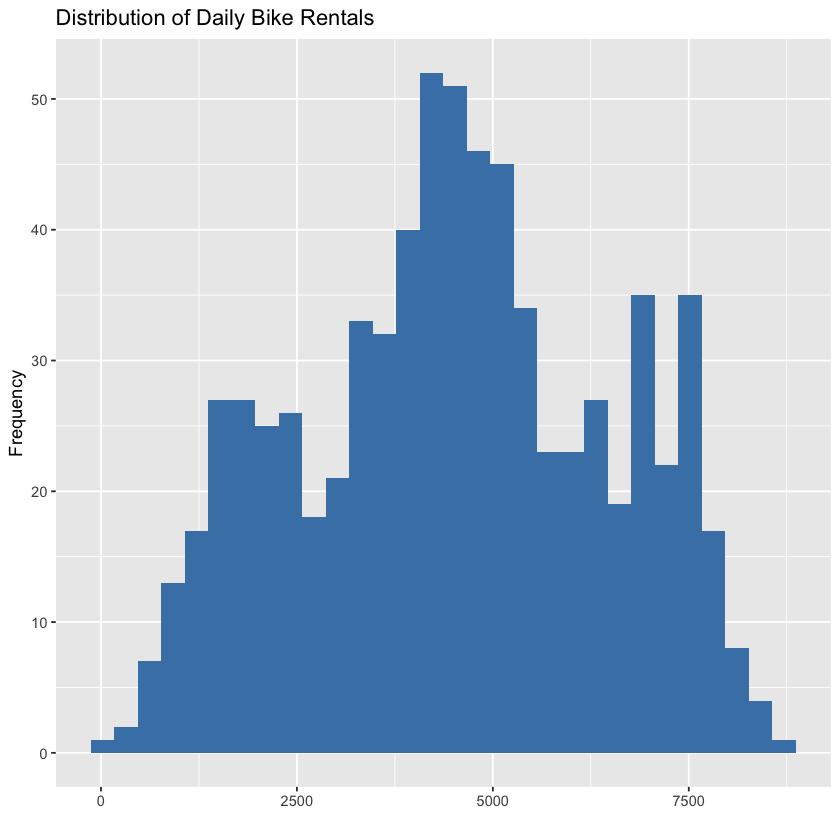
\includegraphics[width=0.7\textwidth]{figures/cnt_distribution.png}
    \caption{Distribution of Daily Bike Rentals}
    \label{fig:cnt_dist}
\end{figure}
 
\subsubsection{Categorical Features}

Figures~\ref{fig:boxplot_season} and~\ref{fig:boxplot_month} show
consistent seasonal trends: counts peak during summer (months 6--9) and
drop substantially in winter (months 1--2), with spring and fall occupying
intermediate levels. The two plots convey near-identical distributional
patterns, reflecting the strong overlap between the two variables.
Figure~\ref{fig:boxplot_yr} shows a marked increase in overall demand from
2011 (Year 0) to 2012 (Year 1), with the median rising from approximately
3,500 to 6,200. A small number of outliers are visible across all three
plots, representing isolated days with unusually low counts; these are
consistent with extreme weather events and are considered a normal
occurrence in the data.


\begin{figure}[H]
    \centering
    \begin{minipage}{0.48\textwidth}
        \centering
        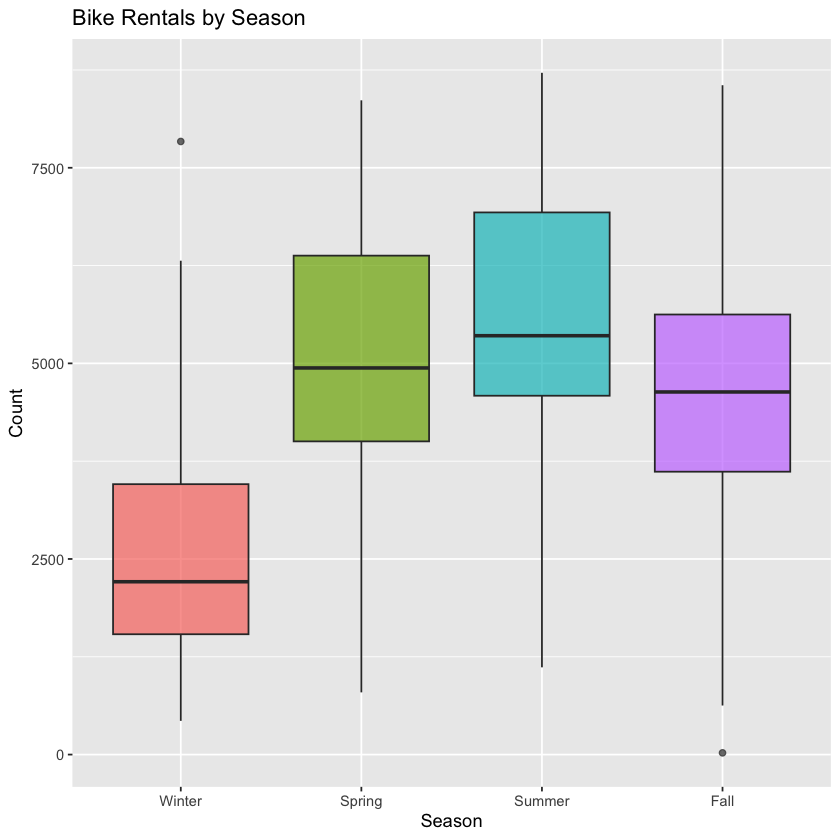
\includegraphics[width=\textwidth]{figures/boxplot_season.png}
        \caption{Bike Rentals by Season}
        \label{fig:boxplot_season}
    \end{minipage}
    \hfill
    \begin{minipage}{0.48\textwidth}
        \centering
        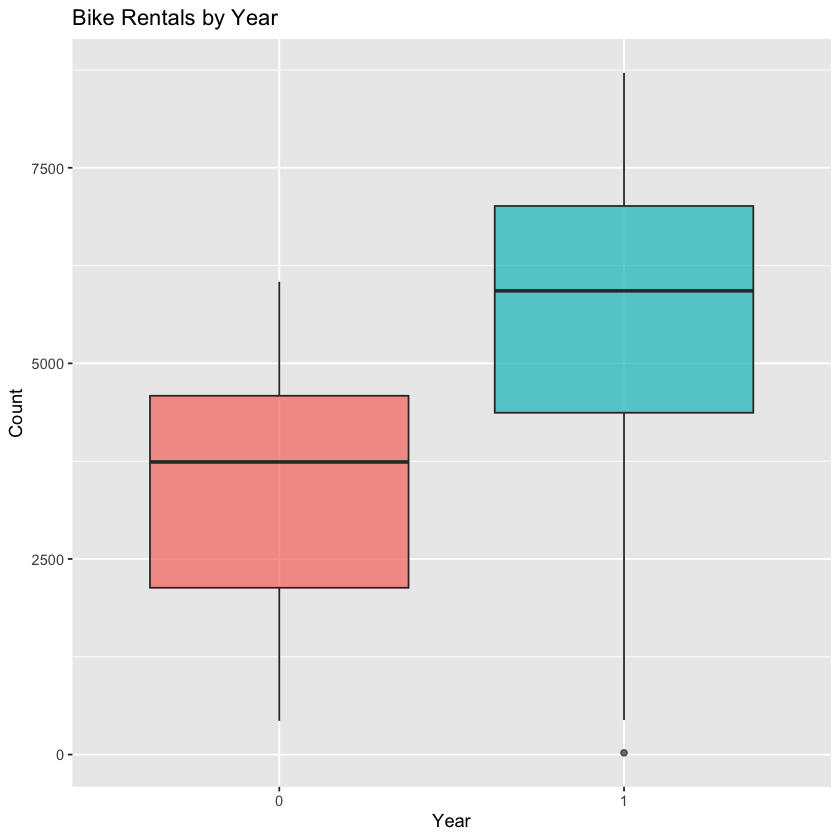
\includegraphics[width=\textwidth]{figures/boxplot_yr.png}
        \caption{Bike Rentals by Year}
        \label{fig:boxplot_yr}
    \end{minipage}
\end{figure}
 
\begin{figure}[H]
    \centering
    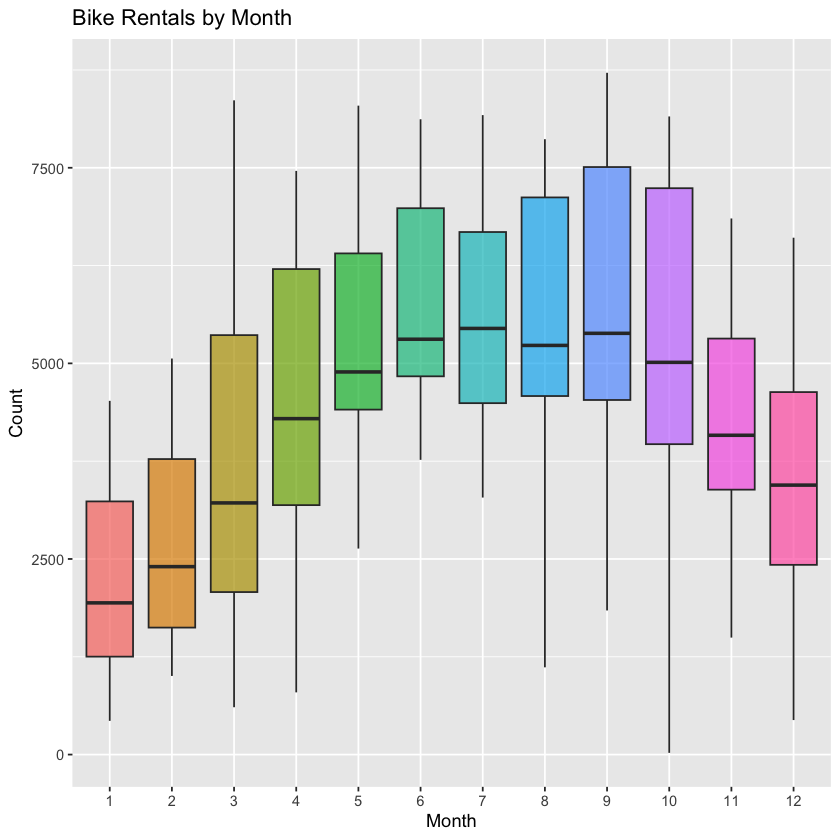
\includegraphics[width=0.6\textwidth]{figures/boxplot_month.png}
    \caption{Bike Rentals by Month}
    \label{fig:boxplot_month}
\end{figure}

Figure~\ref{fig:boxplot_weather} shows rental counts across weather
conditions and day-type indicators. \textit{weathersit} shows a clear
negative trend: higher values indicate more severe weather, and rental
counts decline accordingly. Level 4 does not appear in the dataset as no
such extreme weather days were recorded. \textit{holiday},
\textit{weekday}, and \textit{workingday} show largely overlapping
distributions with no strong separation between categories.

\begin{figure}[H]
    \centering
    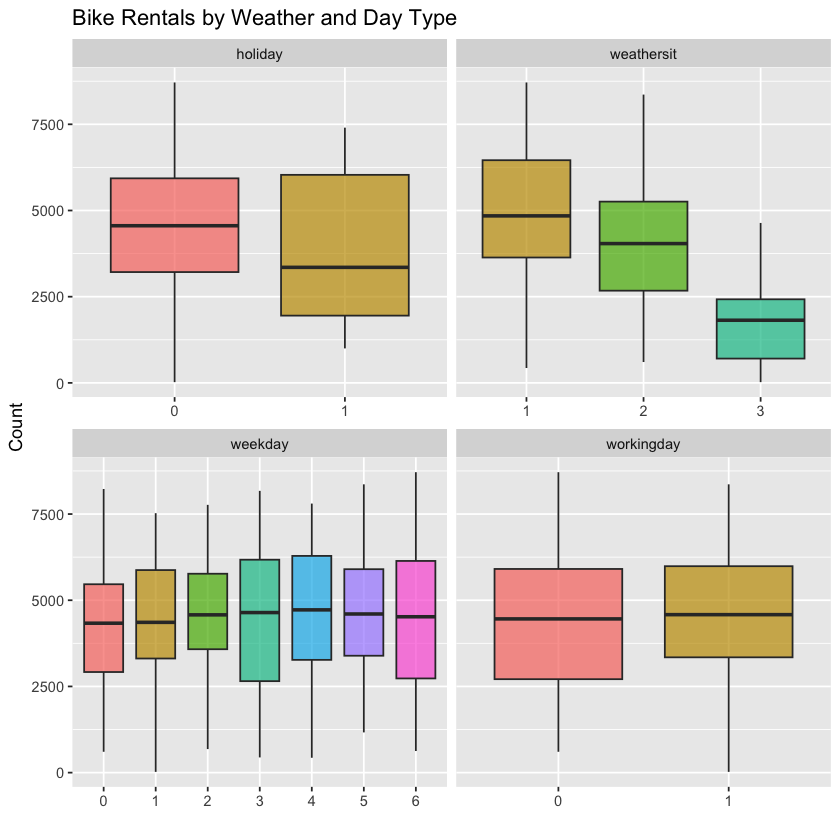
\includegraphics[width=0.55\textwidth]{figures/boxplot_weather_daytype.png}
    \caption{Bike Rentals by Weather and Day Type}
    \label{fig:boxplot_weather}
\end{figure}
 
\subsubsection{Numeric Features}

Figure~\ref{fig:scatter_numeric} shows the relationship between each
numeric feature and daily rental counts. Both \textit{temp} and
\textit{atemp} display near-identical positive trends, suggesting that
the two variables carry largely redundant information. \textit{hum} and
\textit{windspeed} both show negative relationships with rental counts,
indicating that higher humidity and stronger winds are associated with
fewer rentals.

\begin{figure}[H]
    \centering
    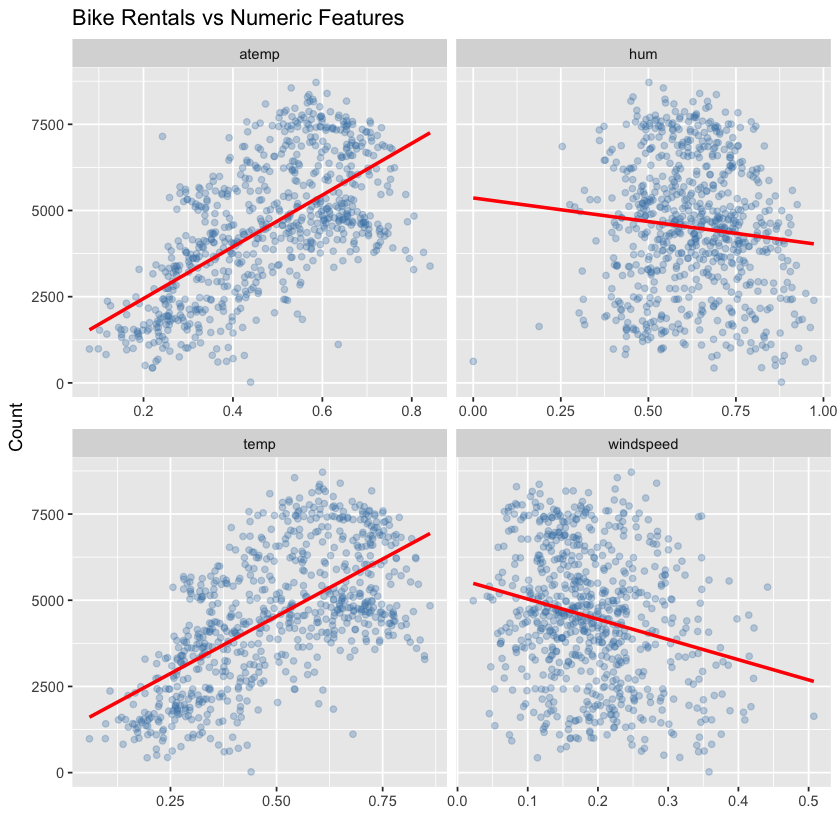
\includegraphics[width=0.55\textwidth]{figures/scatter_numeric.png}
    \caption{Bike Rentals vs Numeric Features}
    \label{fig:scatter_numeric}
\end{figure}

\subsection{Feature Correlation}

Figure~\ref{fig:corr_matrix} shows the correlation matrix for numeric
features. The most notable finding is the near-perfect correlation between
\textit{temp} and \textit{atemp} ($r = 0.99$), confirming the visual
observation from the scatter plots and providing a clear justification for
removing one of the two variables. Both \textit{hum} ($r = -0.10$) and
\textit{windspeed} ($r = -0.23$) show negative correlations with
\textit{cnt}, consistent with the trends observed earlier.

\begin{figure}[H]
    \centering
    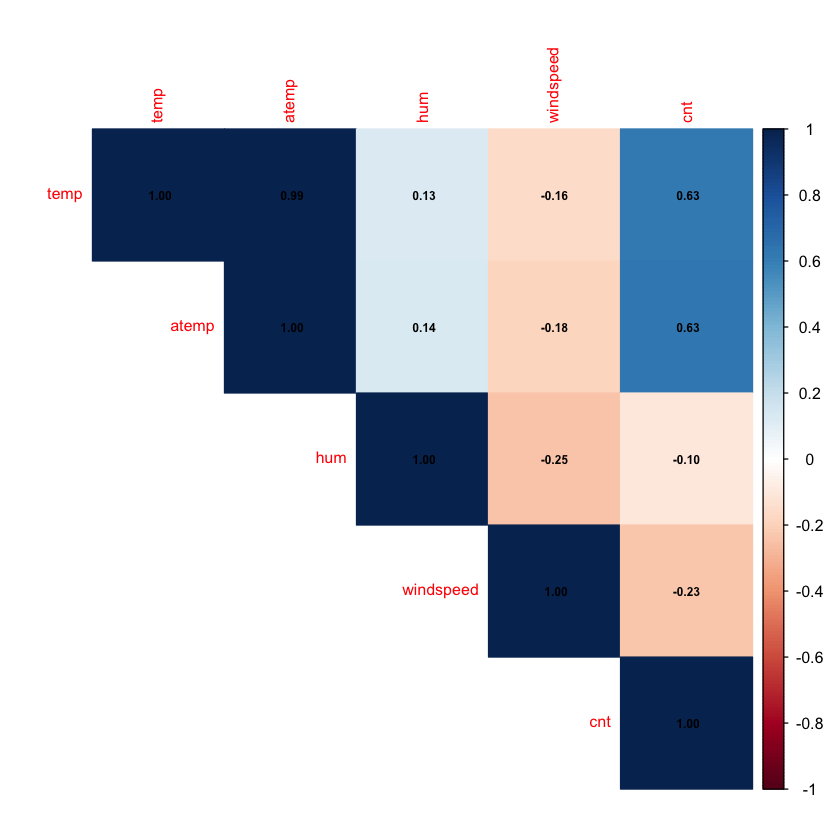
\includegraphics[width=0.7\textwidth]{figures/corr_matrix.png}
    \caption{Correlation Matrix of Numeric Features}
    \label{fig:corr_matrix}
\end{figure}

\subsection{Multicollinearity Check (VIF)}
 
Variance Inflation Factor (VIF) was computed to assess multicollinearity
among the remaining predictors. Before running VIF, three variables were
excluded from the model: \textit{atemp} (near-perfect correlation with
\textit{temp}, $r = 0.99$), \textit{mnth} (aliased with \textit{season}),
and \textit{workingday} (linearly derived from \textit{weekday} and
\textit{holiday}). Including aliased variables causes perfect
multicollinearity, making VIF computation impossible due to a singular
design matrix.
 
All remaining features returned VIF values below 3.6, indicating no
problematic multicollinearity. The two highest values belong to
\textit{season} (3.54) and \textit{temp} (3.41), which reflects a natural
association between temperature and season and does not warrant further
action.
 

%-----------------------------------------------------------------------
\section{Methodology}

\subsection{Ordinary Least Squares (OLS)}
Ordinary Least Squares regression was selected as the primary model for
its interpretability, providing coefficient estimates that directly
quantify the effect of each predictor on daily rental counts. The model
was trained using 5-fold cross-validation to obtain a reliable estimate
of out-of-sample performance.
 
\subsection{Regularisation}

\paragraph{Ridge Regression}
Ridge regression extends OLS by adding an L2 penalty on the magnitude of
coefficients, shrinking them towards zero to reduce variance. It retains
all predictors in the model and is particularly useful when predictors
are correlated. The penalty strength $\lambda$ was selected via 5-fold
cross-validation.
 
\paragraph{Lasso Regression}
Lasso regression applies an L1 penalty, which can shrink some
coefficients to exactly zero, effectively performing feature selection.
Both regularised models use the same cross-validation procedure for
$\lambda$ selection, and serve as a comparison against OLS to evaluate
whether penalisation offers any predictive gain under the current feature
set.

\subsection{Evaluation Metrics}
All three models were evaluated using 5-fold cross-validated RMSE as the
primary metric, and $R^2$ as a supplementary measure of explained
variance. The final models were trained on 8 predictors.
%-----------------------------------------------------------------------
\section{Assumption Diagnostics}
 
\subsection{Residuals vs.\ Fitted}

Figure~\ref{fig:res_fitted} plots residuals against fitted values to
assess linearity and homoscedasticity. Residuals are roughly scattered
around zero with no systematic U-shape or pattern, suggesting that the
linearity assumption is largely satisfied. However, the spread of
residuals appears slightly wider at higher fitted values, indicating mild
heteroscedasticity.

\begin{figure}[H]
    \centering
    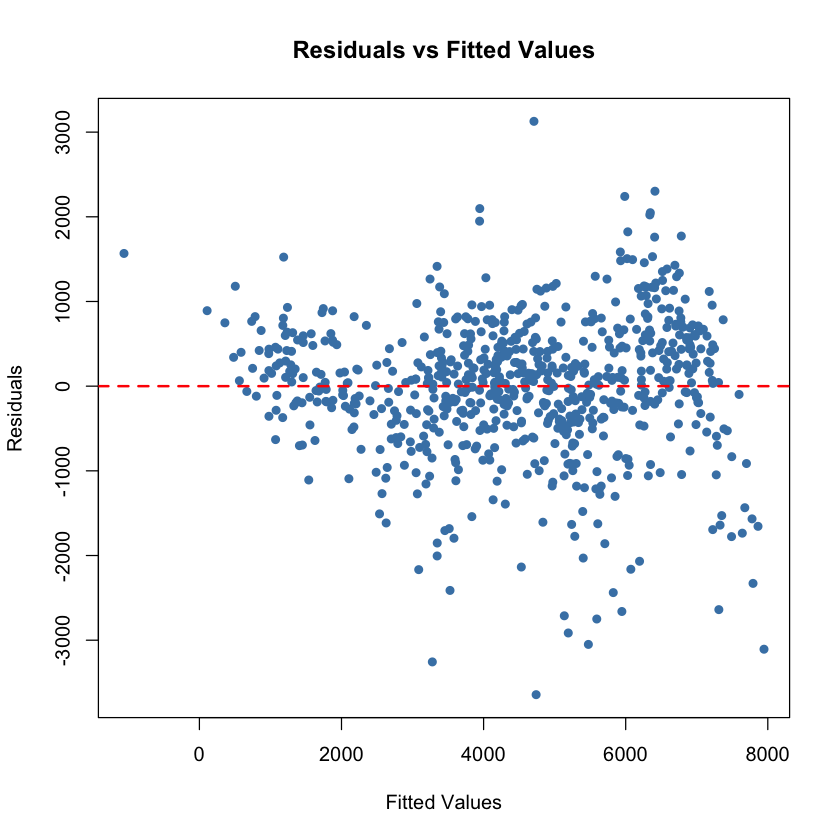
\includegraphics[width=0.5\textwidth]{figures/residuals_vs_fitted.png}
    \caption{Residuals vs.\ Fitted Values}
    \label{fig:res_fitted}
\end{figure}
 
\subsection{Normal Q--Q Plot}

Figure~\ref{fig:qq_plot} compares the distribution of residuals against
a theoretical normal distribution. The middle section follows the
reference line closely, indicating that residuals in the central range
are approximately normally distributed. Both tails deviate from the line,
suggesting slight heavy tails where extreme residuals are more frequent
than a pure normal distribution would predict. One point in the upper
right deviates notably and may represent an outlier. This pattern of
mild leptokurtosis is common in real-world data and does not necessitate
transformation.

\begin{figure}[H]
    \centering
    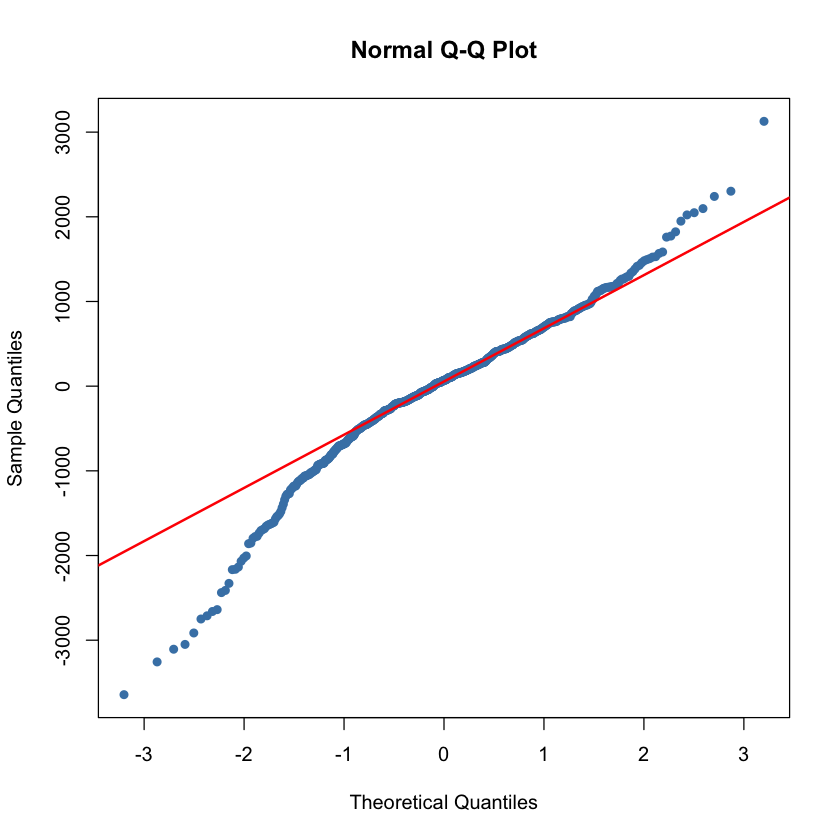
\includegraphics[width=0.55\textwidth]{figures/qq_plot.png}
    \caption{Normal Q--Q Plot of Residuals}
    \label{fig:qq_plot}
\end{figure}
 
\subsection{Scale-Location}

Figure~\ref{fig:scale_loc} plots the square root of standardised residuals
against fitted values to assess homoscedasticity. The red trend line shows
a slight upward slope, indicating that residual variance increases mildly
at higher fitted values. This is consistent with the pattern observed in
the Residuals vs.\ Fitted plot and confirms mild heteroscedasticity,
though the degree is not severe enough to require transformation.
 
\begin{figure}[H]
    \centering
    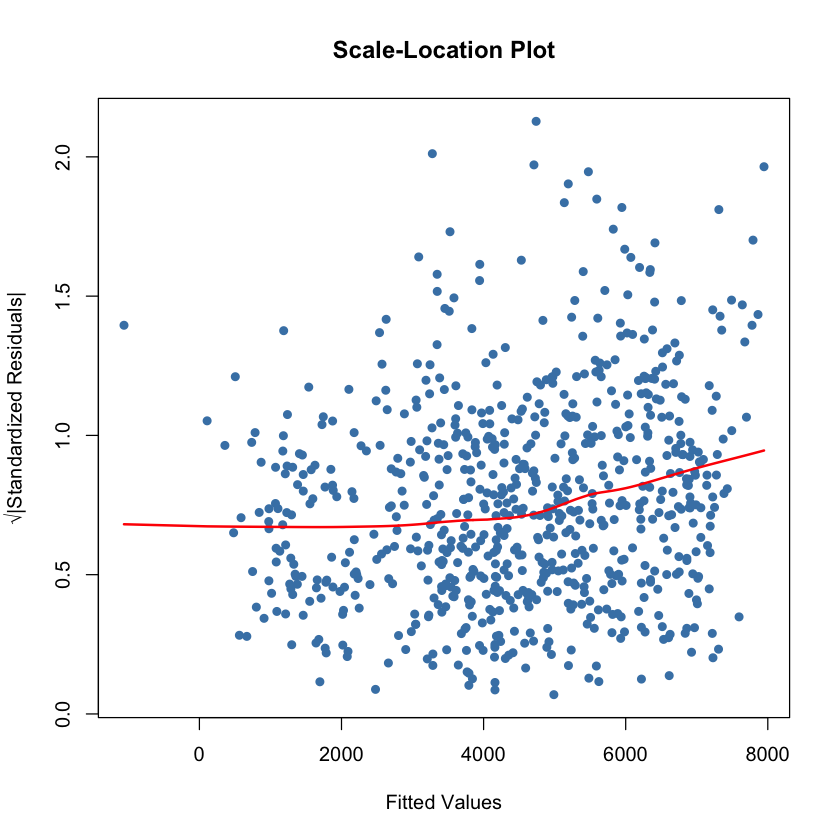
\includegraphics[width=0.55\textwidth]{figures/scale_location.png}
    \caption{Scale-Location Plot}
    \label{fig:scale_loc}
\end{figure}
 
\subsection{Cook's Distance}

Figure~\ref{fig:cooks} shows Cook's Distance for each observation, which
measures how much the model coefficients would change if that observation
were removed. Points exceeding the threshold of $4/n$ (red dashed line)
are considered influential. A total of 39 observations (5.3\%) exceed
this threshold, distributed across the full observation period. This
proportion is within a normal range and does not suggest that the model
is being driven by a small number of anomalous points.
 
\begin{figure}[H]
    \centering
    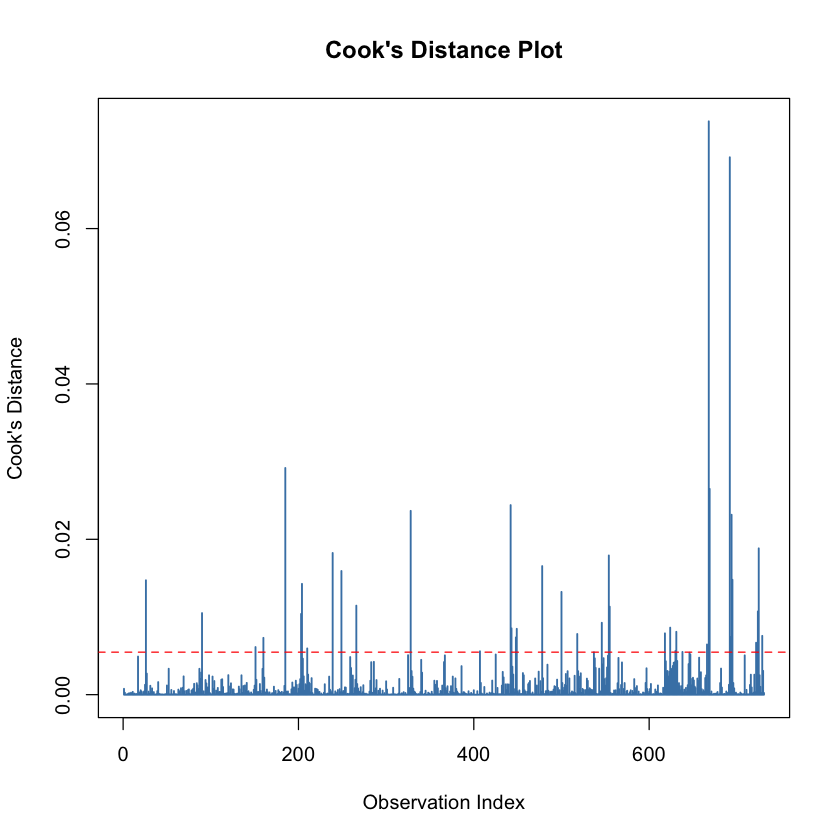
\includegraphics[width=0.55\textwidth]{figures/cooks_distance.png}
    \caption{Cook's Distance}
    \label{fig:cooks}
\end{figure}
 
\subsection{Summary}

Overall, the linear model assumptions are largely satisfied. Linearity
holds with no systematic pattern in the residuals. Mild heteroscedasticity
is present at higher fitted values but is not severe enough to require
transformation. Residuals show slight heavy tails but are approximately
normal in the central range. Influential points account for 5.3\% of
observations, within an acceptable range.

%-----------------------------------------------------------------------
\section{Results}

\subsection{OLS Coefficient Estimates}
 
The OLS model was trained on all 731 observations, achieving an in-sample
$R^2$ of 0.827 and an adjusted $R^2$ of 0.824, indicating that
approximately 82\% of the variance in daily rentals is explained by the
predictors.

Among the predictors, \textit{yr} has the largest effect ($\hat{\beta} = 2017$, $t = 33.0$,
$p < 0.001$), reflecting a strong year-over-year growth trend from 2011
to 2012. \textit{temp} is the strongest continuous predictor
($\hat{\beta} = 5091$, $t = 16.7$, $p < 0.001$), confirming the positive
relationship observed in the EDA. \textit{windspeed} and \textit{hum}
both have significant negative effects, while \textit{weathersit}
deterioration is associated with substantially lower rentals. Among
weekday indicators, \textit{weekday1} is the only non-significant
coefficient ($p = 0.07$), suggesting that Monday demand does not differ
meaningfully from the Sunday baseline.

\subsection{Model Comparison}

Table~\ref{tab:model_compare} compares the three models using
5-fold cross-validated RMSE as the primary metric. OLS achieves the
lowest CV RMSE of 821, outperforming Lasso (831) and Ridge (835).
The marginal difference suggests that regularisation offers limited
improvement when the feature set is already well-specified.
 
\begin{table}[H]
\centering
\caption{Model comparison. CV RMSE is out-of-sample (5-fold
cross-validation); $R^2$ is in-sample.}
\label{tab:model_compare}
\begin{tabular}{lrr}
\toprule
\textbf{Model} & \textbf{CV RMSE} & \textbf{$R^2$} \\
\midrule
OLS   & 821.99 & 0.827 \\
Lasso & 831.18 & 0.827 \\
Ridge & 834.62 & 0.824 \\
\bottomrule
\end{tabular}
\end{table}


%-----------------------------------------------------------------------
\section{Discussion}

\subsection{Key Findings}

 
The OLS model explains approximately 82\% of the variance in daily bike
rentals, with all predictors significant except \textit{weekday1}.
Among all predictors, \textit{yr} emerges as the dominant predictor, capturing a substantial
year-over-year growth in demand from 2011 to 2012. However, this
coefficient reflects a service growth trend rather than a stable seasonal
or behavioural pattern, and may not generalise beyond the observation
period. \textit{temp} is the strongest continuous predictor, reinforcing
the central role of weather conditions in driving rental demand. The
comparison across models shows that OLS outperforms both Ridge and Lasso
on CV RMSE (821 vs 831 vs 835), suggesting that regularisation offers
limited benefit when the feature set is already well-specified through
careful preprocessing.

\subsection{Limitations}

Three limitations are worth noting. First, the model covers only two
years of data, and the large \textit{yr} coefficient may reflect a
growth phase specific to that period rather than a persistent trend,
limiting the model's predictive validity for future years. Second,
prediction errors are likely larger on days with extreme weather
conditions, as such events are rare in the dataset and poorly represented
during training. Third, the model does not include interaction terms,
such as between \textit{temp} and \textit{season}, which may capture
more nuanced demand dynamics and improve predictive performance.

\begin{thebibliography}{9}
 
\bibitem{fanaee2013}
Fanaee-T, H. (2013).
\textit{Bike Sharing} [Dataset].
UCI Machine Learning Repository.
\texttt{https://doi.org/10.24432/C5W894}
 
\end{thebibliography}

\end{document}